\hypertarget{giux1ea3i-phuxe1p-hiux1ec7n-thux1ef1c}{%
\section{Giải pháp hiện
thực}\label{giux1ea3i-phuxe1p-hiux1ec7n-thux1ef1c}}

Chương trình được viết với ngầm định rằng các input của nó (2 số thực
chính xác đơn) sẽ thuộc dạng chuẩn. Các trường hợp khác (subnormal,
infinity, NaN) sẽ không được đảm bảo sẽ tạo ra kết quả chính xác.

Ta biết rằng một sô thực chính xác đơn sẽ có 3 phần - sign, exponent và
fraction. Hướng tiếp cận của chương trình là tách ba phần đó ra từ 2 số,
lưu mỗi phần vào một thanh ghi riêng. Các thanh ghi này được coi là đang
lưu số thực đó dưới dạng trung gian trong lúc xử lí.

Lưu ý đối với chương trình là nó sẽ không xử lí tình huống việc tinh
toán tạo ra kết quả làm overflow hay underflow phần exponent.

Một lưu ý nữa là chương trình sẽ áp dụng chiến thuật làm tròn truncate
(cắt bỏ) - nghĩa là nếu có một bit nào đó bị lọt ra khói khoảng 24 bit
được dùng để chứa phần fraction trong biểu diễn trung gian, nó sẽ bị cắt
bỏ. Chiến thuật làm giúp ta không phải làm tròn kết quả.

\begin{figure}
\centering
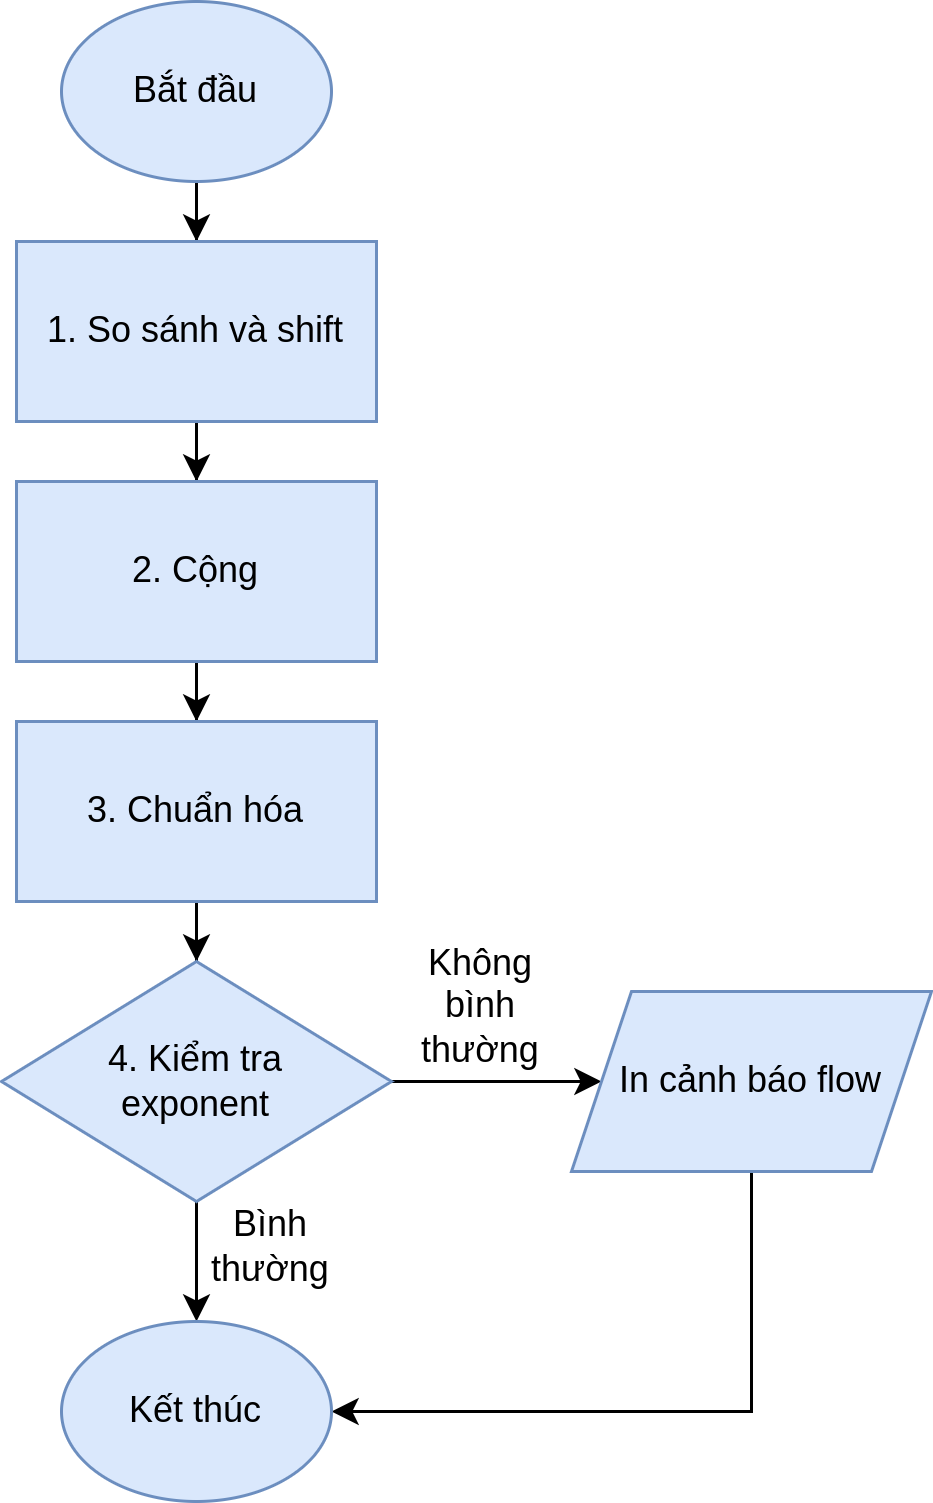
\includegraphics{img/algo_flowchart.png}
\caption{Lưu đồ giải thuật của chương trình}
\end{figure}

Ta liệt kê ra các bước thực hiện tính toán

\begin{enumerate}
\def\labelenumi{\arabic{enumi}.}
\item
  So sánh và dịch dạng trung gian cho tới khi chúng có phần exponent
  bằng nhau
\item
  Cộng phần trung gian
\item
  Chuẩn hóa biểu diễn trung gian (để độ dài còn 24 bit với giá trị bit 1
  ở vị trí 24)
\item
  Kiểm tra underflow và overflow cho exponent sau khi chuẩn hóa
\end{enumerate}

\hypertarget{thux1ed1ng-kuxea-sux1ed1-lux1ec7nh-loux1ea1i-lux1ec7nh-sux1eed-dux1ee5ng-trong-chux1b0ux1a1ng-truxecnh}{%
\section{Thống kê số lệnh, loại lệnh sử dụng trong chương
trình}\label{thux1ed1ng-kuxea-sux1ed1-lux1ec7nh-loux1ea1i-lux1ec7nh-sux1eed-dux1ee5ng-trong-chux1b0ux1a1ng-truxecnh}}

\begin{figure}
\centering
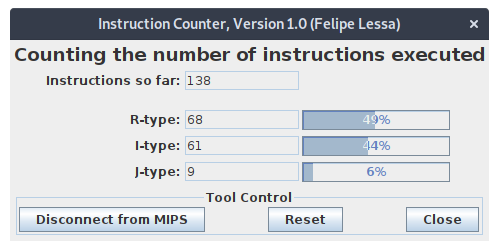
\includegraphics{img/instr_count.png}
\caption{Kết quả từ công cụ thống kê lệnh của MARS}
\end{figure}

Đây là kết quả từ một lần chạy thử của chương trình với đầu vào 100.25
và 0.1. Trong trường hợp lỗi sẽ có xuất hiện thêm một số lượng ít lệnh
nữa. Nhưng ta sẽ coi trung bình số lệnh sẽ rất gần với kết quả thống kê
trên.

Ta có:

\begin{itemize}
\item
  Tổng số lệnh: 138
\item
  Số lệnh dạng R: 68
\item
  Số lệnh dạng I: 61
\item
  Số lệnh dạng J: 9
\end{itemize}

\hypertarget{tuxednh-thux1eddi-gian-chux1ea1y-cux1ee7a-chux1b0ux1a1ng-truxecnh}{%
\section{Tính thời gian chạy của chương
trình}\label{tuxednh-thux1eddi-gian-chux1ea1y-cux1ee7a-chux1b0ux1a1ng-truxecnh}}

Với kết quả số lệnh trên, ta tính toán thời gian thời gian thực hiện
chương trình với bộ xử lý chạy ở xung nhịp CR = 100 Ghz.

Ta cho rằng bộ xử lý này là đơn chu kì (không pileline). Với CPI cho mọi
lệnh bằng 1. Thời gian xử lý có thể được tính

\begin{align*}
\text{Time} &= \text{Clock Period} * \text{Instruction Count}
            &= \frac{1}{CR} * 138
            &= 138 \text{ns}
\end{align*}

\hypertarget{kux1ebft-quux1ea3-kiux1ec3m-thux1eed}{%
\section{Kết quả kiểm thử}\label{kux1ebft-quux1ea3-kiux1ec3m-thux1eed}}

Đây là kết quả từ cùng lần chạy thử với mục thống kê số lệnh.

\begin{figure}
\centering
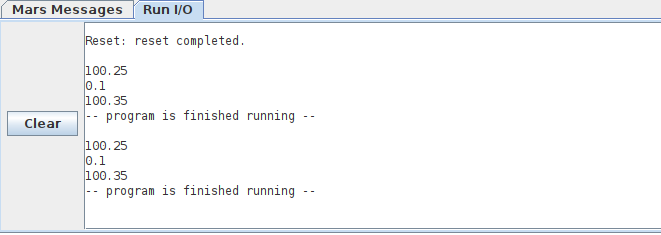
\includegraphics{img/test_result.png}
\caption{Kết quả chạy thử được in ra trong MARS}
\end{figure}
